\subsection{Perencanaan Sistem}

Perencanaan sistem \textit{checkout} otomatis Nasi Padang dilakukan melalui beberapa tahap yang dimulai dari persiapan data hingga model dapat digunakan dalam proses \textit{checkout}. Tahap awal dilakukan dengan mengumpulkan citra Nasi Padang yang memuat objek dari kelas yang akan dikenali. Citra yang telah dikumpulkan kemudian diperiksa dan dipilih agar dapat digunakan sebagai dataset dalam penelitian.

Setiap citra yang digunakan pada proses pelatihan selanjutnya diberikan anotasi untuk menunjukkan kelas dan area dari setiap instans lauk. Anotasi dibuat dalam bentuk \textit{segmentation mask} sehingga setiap objek pada citra memiliki informasi kelas dan batas objek yang digunakan sebagai \textit{ground truth} pada proses pelatihan YOLO11-seg.

Dataset yang telah dianotasi kemudian dibagi menjadi data pelatihan, validasi, dan pengujian. Pembagian dilakukan sebelum proses augmentasi agar citra hasil augmentasi tidak tersebar pada bagian dataset yang berbeda. Augmentasi hanya diterapkan pada data pelatihan untuk menambah variasi citra yang digunakan selama proses pembelajaran model \cite{yang2022augmentation,tampu2022}.

Data pelatihan selanjutnya digunakan untuk melatih YOLO11-seg. Pada proses pelatihan, model menerima citra beserta \textit{ground truth} dan menghasilkan prediksi lokasi objek, kelas, serta \textit{segmentation mask}. Hasil prediksi dibandingkan dengan \textit{ground truth} untuk memperoleh nilai \textit{loss}, kemudian bobot model diperbarui melalui proses \textit{backpropagation}. Proses tersebut dilakukan secara berulang hingga diperoleh model akhir yang digunakan pada tahap inferensi.

Pada tahap inferensi, citra piring yang diperoleh dari kamera diberikan kepada model yang telah dilatih. Model menghasilkan sejumlah instans objek yang masing-masing memiliki informasi kelas dan \textit{segmentation mask}. Setiap instans yang dikenali kemudian dihitung berdasarkan kelasnya sehingga diperoleh jumlah lauk dari masing-masing kelas.

Hasil penghitungan tersebut selanjutnya diteruskan ke program kalkulasi harga. Program mencocokkan setiap kelas lauk dengan harga tetap yang telah ditentukan, kemudian menghitung subtotal berdasarkan jumlah instans pada kelas tersebut. Seluruh subtotal dijumlahkan untuk menghasilkan total harga yang harus dibayarkan pada proses \textit{checkout}.

Tahap persiapan dataset yang digunakan dalam perencanaan sistem dijelaskan lebih lanjut pada subbagian berikut.

\subsubsection{Pengumpulan Data}

Tahap pengumpulan data dilakukan untuk memperoleh citra Nasi Padang yang akan digunakan dalam proses pelatihan dan pengujian model YOLO11-seg. Data yang dikumpulkan berupa citra piring Nasi Padang yang memuat satu atau lebih lauk dari kelas yang digunakan dalam penelitian.

Pengumpulan citra dilakukan melalui dua sumber, yaitu pengambilan citra secara langsung dan pengumpulan citra dari internet. Pengambilan citra secara langsung dilakukan untuk memperoleh citra yang sesuai dengan kondisi penggunaan sistem, sedangkan citra dari internet digunakan untuk menambah variasi tampilan lauk, seperti bentuk, penyajian, posisi objek, dan kondisi pencahayaan.

Citra yang dikumpulkan kemudian melalui proses seleksi sebelum digunakan sebagai dataset. Citra yang tidak menampilkan objek dengan cukup jelas, memiliki kualitas yang terlalu rendah, merupakan duplikat, atau memiliki elemen visual yang menutupi sebagian besar objek tidak digunakan. Seleksi tersebut dilakukan agar citra yang digunakan tetap memberikan informasi visual yang memadai untuk proses anotasi dan pelatihan model.

Dataset difokuskan pada sembilan kelas yang digunakan dalam sistem, yaitu nasi, rendang, ayam goreng, perkedel, sayur nangka, daun singkong, telur dadar, telur kari, dan sambal. Satu citra dapat mengandung lebih dari satu kelas maupun lebih dari satu instans dari kelas yang sama. Kondisi tersebut diperlukan karena pada penggunaan sistem, satu piring dapat berisi beberapa jenis lauk secara bersamaan.

Selain citra dengan objek yang terlihat secara terpisah, dataset juga dapat memuat citra dengan kondisi objek saling bersentuhan atau mengalami oklusi. Kondisi oklusi tidak diasumsikan dapat diselesaikan sepenuhnya oleh model, tetapi digunakan sebagai salah satu kondisi yang akan dievaluasi untuk mengetahui perubahan performa YOLO11-seg dibandingkan dengan kondisi non-oklusi.

Citra yang telah lolos proses seleksi selanjutnya digunakan pada tahap anotasi. Setiap objek yang termasuk dalam sembilan kelas penelitian akan diberikan anotasi kelas dan area segmentasi sehingga dapat digunakan sebagai \textit{ground truth} dalam proses pelatihan YOLO11-seg.

Contoh citra yang digunakan dalam dataset ditunjukkan pada Gambar~\ref{fig:contoh-dataset}.

\begin{figure}[H]
    \centering
    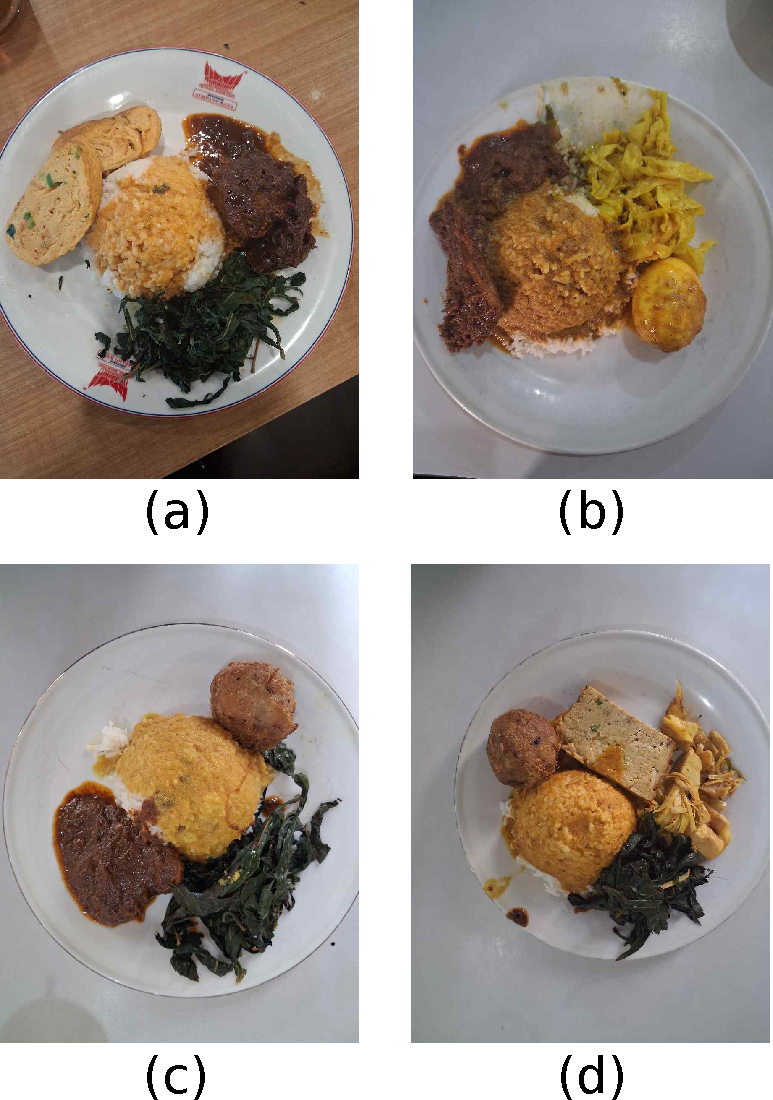
\includegraphics[width=0.55\textwidth]{figures/contoh_dataset.pdf}
		\caption{Contoh citra hasil pengumpulan data secara langsung}
    \label{fig:contoh-dataset}
\end{figure}

\subsubsection{Anotasi Data}

Citra yang telah lolos tahap seleksi dianotasi untuk menghasilkan \textit{ground truth} yang diperlukan dalam pelatihan, validasi, dan pengujian YOLO11-seg. Anotasi dilakukan pada setiap instans objek makanan yang termasuk dalam kelas penelitian menggunakan CVAT.

Anotasi dibuat dalam bentuk poligon yang mengikuti batas objek yang terlihat pada citra. Setiap poligon diberikan label kelas sehingga memuat informasi mengenai jenis dan area objek. Apabila satu citra mengandung lebih dari satu instans dari kelas yang sama, setiap instans dianotasi secara terpisah agar model dapat mempelajari dan menghasilkan \textit{segmentation mask} untuk setiap instans secara individual.

Kelas yang digunakan dalam proses anotasi terdiri atas nasi, rendang, ayam goreng, perkedel, sayur nangka, daun singkong, telur dadar, telur kari, dan sambal. Objek makanan di luar sembilan kelas tersebut tidak diberikan anotasi dan diperlakukan sebagai bagian dari latar belakang.

Pada objek yang mengalami oklusi, poligon mengikuti batas bagian objek yang masih terlihat tanpa memperkirakan area yang tertutup oleh objek lain. Ketentuan ini digunakan agar anotasi tetap didasarkan pada informasi visual yang tersedia pada citra.

Anotasi yang telah dibuat diperiksa kembali untuk memastikan kesesuaian label kelas, ketepatan poligon terhadap batas objek, dan pemisahan setiap instans. Hasil anotasi kemudian disimpan dalam format yang sesuai dengan kebutuhan YOLO11-seg dan digunakan pada tahap pembagian dataset.

\subsubsection{Pembagian Dataset}

Dataset yang telah dianotasi selanjutnya dibagi menjadi data pelatihan, validasi, dan pengujian. Pembagian tersebut dilakukan agar proses pelatihan dan evaluasi menggunakan bagian dataset yang berbeda.

Dataset dibagi dengan proporsi 70\% untuk data pelatihan, 15\% untuk data validasi, dan 15\% untuk data pengujian. Jumlah citra pada setiap bagian ditentukan berdasarkan jumlah akhir citra yang telah lolos tahap seleksi dan anotasi. Pembagian dilakukan dengan memperhatikan keterwakilan sembilan kelas penelitian pada setiap bagian dataset.

Data pelatihan digunakan dalam proses pembelajaran dan pembaruan bobot YOLO11-seg. Data validasi digunakan untuk memantau performa model selama pelatihan dan membantu menentukan model terbaik. Data pengujian disimpan secara terpisah dan hanya digunakan untuk mengevaluasi performa model akhir pada citra yang tidak digunakan dalam proses pelatihan.

Pembagian dataset dilakukan sebelum proses augmentasi untuk mencegah citra asli dan hasil augmentasinya tersebar pada bagian dataset yang berbeda. Citra duplikat, citra yang memiliki kemiripan tinggi, dan citra yang berasal dari sumber dasar yang sama ditempatkan pada bagian dataset yang sama untuk mengurangi risiko kebocoran data \cite{tampu2022}. Augmentasi selanjutnya hanya diterapkan pada data pelatihan.

\subsubsection{Augmentasi Data}

Augmentasi diterapkan pada data pelatihan untuk menambah variasi data yang diterima model selama proses pembelajaran. Penerapan augmentasi bertujuan membantu model mempelajari variasi tampilan objek dan mengurangi kecenderungan model menghafal karakteristik citra tertentu \cite{yang2022}.

Augmentasi dilakukan secara dinamis melalui \textit{pipeline} pelatihan YOLO11-seg. Dengan mekanisme ini, transformasi dapat diberikan ketika data pelatihan dimuat tanpa harus menghasilkan salinan citra baru secara permanen. Transformasi pada citra juga diterapkan pada anotasi sehingga posisi \textit{segmentation mask} tetap sesuai dengan objek setelah augmentasi.

Jenis transformasi dipilih dengan mempertimbangkan karakteristik citra dan kondisi penggunaan sistem. Transformasi dapat mencakup perubahan posisi, skala, orientasi, serta karakteristik warna dan pencahayaan selama transformasi tersebut tidak mengubah identitas utama objek atau menghasilkan kondisi yang tidak relevan terhadap penggunaan sistem.

Augmentasi acak tidak diterapkan pada data validasi dan pengujian agar kedua bagian tersebut tetap digunakan sebagai data evaluasi yang merepresentasikan citra aslinya. Konfigurasi augmentasi yang benar-benar digunakan pada proses pelatihan dicatat pada tahap pembuatan sistem.

